
\noindent En este capítulo se aborda el análisis de malware, en qué consiste, su importancia y los tres tipos de análisis que existen: el estático \ref{sec:aestatico}, el dinámico \ref{sec:adinamico} y el híbrido \ref{sec:ahibrido} . El capítulo termina explicando el aprendizaje automático aplicado al análisis de malware \ref{sec:mlaplicado} y los algoritmos más usados para el desarrollo de modelos que detecten automáticamente las amenazas. 



\section{Introducción}

\noindent El análisis de malware es el estudio del comportamiento del malware, y su objetivo es comprender el funcionamiento del malware, sus capacidades, cómo detectarlo, contenerlo y/o eliminarlo \cite{113}. Esto implica analizar el programa sospechoso en un entorno seguro para identificar sus características y así poder construir mejores defensas para defender la red de una empresa. Además, analizar malware sirve para encontrar vulnerabilidades en nuestros sistemas, nuevos métodos de infección y la evolución de los atacantes y sus propósitos \cite{LMA2018}.
Las razones por las que es importante realizar un análisis de malware son \cite{75}:
\begin{itemize}
\item Determinar la naturaleza y finalidad del malware. Es importante saber si el malware es un ransomware, un \textit{spyware} \cite{114}, un \textit{rootkit} \cite{115}, un \gls{RAT} \cite{116}, etc.
\item Entender cómo se vio comprometido el sistema y el impacto que tuvo el malware sobe él \cite{118}.
\item Encontrar los indicadores de red del malware mediante la monitorización de la red. Estos indicadores se utilizan para detectar infecciones parecidas. Por ejemplo, si durante el análisis se concluye que un malware contacta con una dirección \gls{IP} en particular, se puede monitorizar el tráfico de la red para identificar todos los equipos que contactan con esa dirección.
\item Extraer conclusiones como claves de registro y nombres de archivo basándonos en el equipo. También se utilizan para detectar una infección parecida en otro equipo. Por ejemplo, si un malware crea una clave de registro, se puede utilizar esa misma clave como indicador para identificar todos los equipos que tienen la misma clave de registro.
\item Determinar el motivo del atacante, su intención y su identidad si es posible para poder clasificar el malware correctamente. 
\end{itemize}

Para comprender el funcionamiento y las características del malware y evaluar su impacto en los sistemas que infecta, se utilizan tres tipos de análisis: estático, dinámico e híbrido. 


%Las principales metodologías de análisis de malware son el análisis estático (no ejecuta el malware) y el análisis dinámico (observa el comportamiento del malware mientras actúa).



\section{Análisis Estático}
\label{sec:aestatico}

\noindent El análisis estático de una muestra de malware consiste en analizar un binario en busca de signos de intenciones maliciosas sin tener que ejecutarlo \cite{111}, es decir, poder determinar si se trata de una muestra maliciosa antes de que comience a actuar, incluso es posible encontrar más información acerca del tipo y familia de malware y el comportamiento que tendrá \cite{Mohanta2020}. Es más fácil de realizar y permite extraer los metadatos asociados con el programa sospechoso.
Este tipo de análisis se puede interpretar como una ``disección'' del binario sin el riesgo de que el malware actúe en nuestro equipo \cite{EPN2014}.

A la hora de realizar análisis estático de una muestra, se utiliza principalmente un desensamblador para realizar la “disección” anteriormente mencionada y decodificar el código máquina del malware \cite{SIM2020}.

Puede que el análisis estático no revele toda la información necesaria, pero puede proporcionar información interesante que ayude a determinar el enfoque de los análisis posteriores. Para determinar si un archivo es malicioso, se usan indicadores técnicos denominados \gls{IoC} como nombres de archivo, direcciones \gls{IP}, dominios y datos en el encabezado del archivo \cite{90}, y herramientas como analizadores de red para observar el malware sin ejecutarlo para recopilar información sobre cómo funciona \cite{113}. 


\subsection{Técnicas}

\noindent La elección de la técnica para revelar información de un archivo potencialmente malicioso depende del objetivo y del contexto que rodea al archivo sospechoso \cite{89}. Algunas de las técnicas o fases de análisis estático son:

\begin{itemize}
    \item \textbf{Determinar el tipo de fichero y arquitectura}: La extensión del binario ayuda a averiguar cual es la máquina objetivo del malware (Windows, MacOS, etc.) y la arquitectura del mismo. Por ejemplo, si el tipo del archivo es \gls{PE}, que es el formato de archivo para los ejecutables de Windows (.exe, .dll, .sys, .drv, .com, .ocx, etc) \cite{96}, entonces se puede deducir por la extensión del archivo que el malware está diseñado para atacar el sistema operativo Windows.
    Aun así, esto no es del todo fiable ya que los atacantes utilizan diferentes trucos para ocultar el archivo, modificar la extensión real del fichero y cambiar su apariencia con el fin de engañar a los usuarios para que lo ejecuten.
    Para encontrar la extensión real de un fichero en Windows, es posible fijarse en la firma del mismo (\textit{file signature}). Una firma de archivo es una secuencia única de bytes que se escribe en su encabezado \cite{97}. los primeros bits indicarán si se trata de algún tipo de ejecutable (\gls{PE} files). Esto se puede determinar utilizando métodos manuales o herramientas específicas \cite{LMA2018}. 
    También es posible determinar si se está falseando la extensión o se trata de un archivo sospechoso prestando atención a sus propiedades (información o detalles de la versión, copyright de la aplicación, etc.) o con una aplicación específica, como CFF Explorer, para observar si la miniatura del archivo ha sido modificada para simular ser un fichero legítimo \cite{Mohanta2020}.

    \item \textbf{Huellas digital del malware}: Esta técnica consiste en la generación del \textit{hash} criptográfico para los binarios basándose en el contenido del fichero \cite{LMA2018}. Los algoritmos más comunes son MD5, SHA1 y SHA256 y a la hora de realizar un análisis es bueno generar los tres tipos de \textit{hashes} para la misma muestra. El motivo de generar el hash para una muestra es que podemos compartir esta información con plataformas de análisis u otros usuarios para identificar el malware sin tener que compartir el mismo, evitando infectar un equipo ajeno o transmitir información personal del usuario \cite{Mohanta2020}.La generación de estos valores \textit{hash} se realiza mediante la ejecución los comandos \textit{md5sum}, \textit{sha256sum} y \textit{sha1sum} en Linux o mediante el uso del módulo \textit{hashlib} en Python.


    \item \textbf{Inspección de la información del encabezado \gls{PE}}: La cabecera de un archivo, además de contener su tipo, incluye información sobre dónde se debe cargar el ejecutable en la memoria, la dirección donde comienza la ejecución, la lista de bibliotecas y funciones en las que se basa la aplicación y los recursos utilizados \cite{86}. Para realizar tales interacciones, el malware depende de las funciones del sistema operativo. Windows exporta estas funciones llamadas \gls{API} en archivos \gls{DLL} (archivos pertenecientes a bibliotecas de enlaces dinámicos) \cite{103}. Los ejecutables importan y llaman a estas funciones normalmente desde varios archivos \gls{DLL} que proporcionan diferentes funcionalidades. La inspección de los archivos \gls{DLL} en las que se basa un malware y las funciones \gls{API} que importa pueden dar una idea sobre la funcionalidad y capacidad del malware. Toda esta información de las importaciones se almacena en tablas en el encabezado \gls{PE} \cite{75}.

    \item \textbf{Escaneo del virus con un programa específico como un antivirus}: Realizar esta acción ayuda a saber más acerca de la posible muestra maliciosa y mejorar nuestro análisis \cite{LMA2018}. Para ello, se suele utilizar algún antivirus específico que instalado en el equipo o en páginas web como VirusTotal o Jotti Virus Scan, que ofrecen un servicio de escaneo de malware con varias fuentes con el fin de determinar la peligrosidad de una muestra y almacenan toda la información obtenida a la cual se puede acceder y se comparte con empresas u organizaciones interesadas. Además, existen otras plataformas web como “file2scan” o “scan4you” las cuales son de pago y no comparten la información con nadie, siendo el escaneo anónimo, lo que permite a cibercriminales comprobar la peligrosidad de sus archivos maliciosos \cite{EPN2014} \cite{LMA2018}. El riesgo que existe en esta técnica es que el escaneo no detecte el fin malicioso de la muestra, pero aún así, siga tratándose de un malware.
    
    \item \textbf{Detectar protección o empaquetadores}: Los creadores de malware en su mayoría buscan ocultar el contenido y funcionamiento del malware para que en el análisis del mismo sea difícil o imposible encontrar esta información. Para realizar esto, se utilizan programas específicos conocidos como empaquetadores o \textit{packers} o \textit{cryptors} \cite{EPN2014}. Los empaquetadores o packers ocultan el ejecutable en un nuevo archivo que cuando se activa, “descomprime” el binario original para realizar el ataque. El \textit{cryptor} es parecido, pero utiliza cifrado en lugar de compresión \cite{LMA2018}. Para detectar este tipo de empaquetado o cifrado, se pueden utilizar herramientas como Exeinfo PE,  PEiD o RDG Packer Detector.
    
    \item \textbf{Extracción de cadenas, funciones y metadatos asociados con el binario}: Las cadenas son secuencias de caracteres en \gls{ASCII} y \textit{Unicode} contenidas en un archivo \cite{101}. La extracción de estas cadenas  puede dar pistas sobre la funcionalidad del programa, ya que contienen referencias a nombres de archivo, varias \gls{URL}, nombres de dominio, direcciones \gls{IP}, comandos de ataque, claves de registro, etc. Aunque las cadenas no dan una imagen clara del propósito y la capacidad de un malware, puede ayudar a encontrar información sobre la acción del fichero malicioso o sobre el atacante, como por ejemplo el tipo de malware, direcciones \gls{IP}, comandos de ataque, claves, objetivos del malware, etc. \cite{LMA2018}. Para extraer estas cadenas, existe un comando en Linux llamado \textit{strings}, pero esto sólo es posible si la información no ha sido ocultada mediante \textit{packers} o \textit{cryptors} o si estos han empleado una protección vulnerable. Para estos casos se puede usar la herramienta \textit{pestudio} para extraer cadenas de un binario sospechoso o a \gls{FLOSS} para detectar y extraer información oculta \cite{102}.
    
    \item \textbf{Clasificación de las muestras}: Con el fin de conocer características específicas de un malware o su pertenencia, se compara el binario con otras muestras analizadas previamente o almacenadas en un repositorio que puede ser privado o público. El \textit{hash} criptográfico visto anteriormente es una gran técnica para detectar muestras idénticas, pero no ayuda a identificar muestras similares ya que a menudo los delincuentes cambian ciertos parámetros del malware que modifican el \textit{hash} por completo y dificulta esta tarea. Para poder clasificar las muestras de malware se pueden utilizar técnicas como \textit{Fuzzy Hashing} (mediante la herramienta \textit{ssdeep}) \cite{104}, \textit{Import Hash} (que mira las funciones \gls{API} llamadas por los dos archivos)  \cite{105} o YARA (una herramienta para crear reglas que consisten en expresiones booleanas y cadenas basadas en patrones de información del binario para poder identificarlo cuya complejidad puede ser muy alta) \cite{YARADOC} \cite{77}. 
\end{itemize}

En la Figura \ref{fig:staticFlow} se muestra el diagrama de flujo del proceso de un análisis estático, mencionando todas las técnicas explicadas anteriormente.

\begin{figure}[h!]
\begin{center}
{\scalebox{.3}{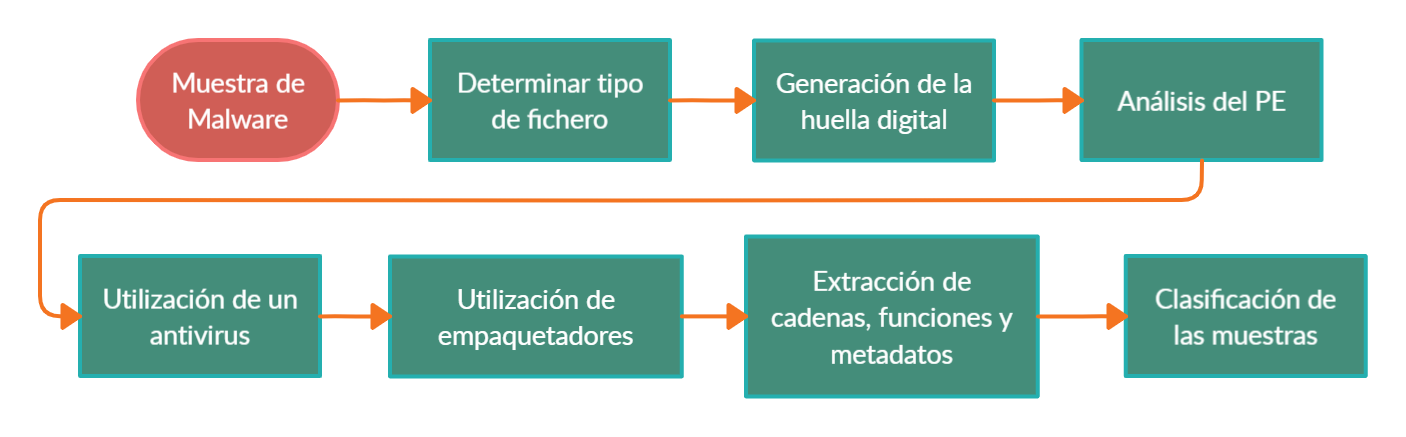
\includegraphics{images/static-flow.png}}}
\end{center}
\caption{Diagrama de flujo de un análisis estático.}
\label{fig:staticFlow}
\end{figure}

El problema del análisis estático es que, al no ejecutar el código, un malware más sofisticado puede incluir comportamientos maliciosos en tiempo de ejecución que pueden pasar desapercibidos. Por ejemplo, si descarga un archivo malicioso basado en una cadena dinámica, el análisis estático no lo detectará \cite{117}. Es por esto por lo que las empresas recurren al análisis dinámico para una comprensión más completa del comportamiento del malware.

\subsection{Herramientas}

\noindent Existen diferentes herramientas de análisis estático según la técnica que apliquen, algunas de las más conocidas y usadas se muestran en la Tabla \ref{tab:toolsEst}.

\begin{table}[htb!]
\centering
\scriptsize %para hacer la tabla mas pequeña
\caption{Herramientas de análisis estático}
\begin{tabular}{|l|p{12cm}|}
\hline
\rowcolor[HTML]{C0C0C0}
\multicolumn{1}{|c|}{\cellcolor[HTML]{C0C0C0}{\textbf{Herramienta}}} & \multicolumn{1}{c|}{\cellcolor[HTML]{C0C0C0}{\color[HTML]{000000} \textbf{Descripción}}}\\ \hline

    \textbf{WinMD5Free}& Una herramienta gratuita con interfaz gráfica para calcular el \textit{hash} de un fichero utilizando el algoritmo \gls{MD5} para comprobar comparando el \textit{hash} generado si el fichero ha sido alterado en algún momento \cite{EPN2014}.\\ \hline
    
    \textbf{CFF Explorer}& Un conjunto de herramientas gratuitas destinado a la monitorización de procesos y la edición de ficheros \gls{PE} que permite la modificación de campos especiales, incluye desensamblador y gestión de firmas entre otras muchas funcionalidades \cite{EPN2014}.\\ \hline

    \textbf{Ollydbg}& Un simple depurador sólo para sistemas Windows de 32 bits enfocado principalmente al análisis de código binario. Las diferentes características de este programa permiten usar \textit{breakpoints} y cambiar instrucciones y condiciones en el ejecutable, además, es libre y no necesita instalación. Destaca también por tener una gran variedad de \textit{plugins} \cite{Vokorokos2017}.\\ \hline
    
    \textbf{Ghidra}&Herramienta desarrollada en Java analiza tanto ficheros \gls{PE} como \gls{ELF} y puede utilizarse en Windows, Linux y MacOS. Se trata de un proyecto desarrollado por la \gls{NSA} de Estados Unidos que, además de desensamblar binarios, contiene un decompilador para sacar un pseudocódigo en lenguaje C del fichero analizado \cite{SIM2020}.\\ \hline
    
    \textbf{IDA Pro}& Es un proyecto de Hex-Rays utilizado para ingeniería inversa del cual se puede obtener una versión básica con pocas funcionalidades gratuitamente. Básicamente, \gls{IDA} Pro es un sofisticado desensamblador con múltiples funcionalidades en su versión completa que busca hacer el código complejo más legible para el usuario \cite{IDA2011}.\\ \hline
    
     \textbf{Radare2}& Un proyecto libre el cual se puede obtener de un repositorio en GitHub y está basado en un conjunto de comandos que se pueden usar juntos o aislados. Cuenta con diferentes programas como rabin2, rasm2, rahash2… siendo el principal de todos radare2, que permite “diseccionar” un binario, analizar los datos, desensamblar el código, etc. Además, admite diferentes lenguajes, entre ellos Python, JavaScript o Perl \cite{RAD2ORG}. \\ \hline
    
    \textbf{PEiD}& Una de las herramientas más usada en todo el mundo para identificar \textit{packers} ya que es la que mejores resultados ha proporcionado. 
    Una de las claves de su éxito es que contiene un alto número de firmas de empaquetadores para identificar a estos. Además, es gratuita \cite{Kancherla2015}.\\ \hline
    
    \textbf{PEStudio}& Una sencilla aplicación libre usada para estudiar cualquier tipo de ejecutable extrayendo cadenas y firmas. Los resultados son similares a los que ofrece VirusTotal, lo que permite complementar la herramienta \cite{Amiruddin2020}.\\ \hline
\end{tabular}
\label{tab:toolsEst}
\end{table}

\subsection{Limitaciones}

\noindent Este tipo de análisis muchas veces no sirve para encontrar una resolución clara y es necesario cambiar de técnica si se quiere llegar a algún tipo de resultado. En definitiva el análisis estático sirve para encontrar información sobre la muestra y que esta ayude en una siguiente fase \cite{Mohanta2020}, además, este análisis puede ser muy complicado debido a que el código ensamblador sea ilegible, ya que algunas funciones las codifican y para poder leerlo sea necesario ejecutar el binario, por lo que ya se hablaría de análisis dinámico \cite{SIM2020}.

\section{Análisis Dinámico} \label{sec:adinamico}

\noindent El análisis dinámico de una muestra se realiza mientras que esta está siendo ejecutada y es más importante que nunca hacerlo en un entorno controlado montando un laboratorio de análisis \cite{111}.  Esta técnica de ejecutar el programa malicioso en un entorno seguro se conoce como \textit{sandboxing} \cite{122}, o aislamiento de procesos en español.  En este tipo de análisis se presta atención a las llamadas a \gls{API}, el tráfico de red o la actividad en procesos, en archivos o en el registro del sistema \cite{Gandotra2014}.
Para realizar el análisis dinámico se pueden utilizar tanto herramientas instaladas en un equipo como plataformas web que ahorran el trabajo de montar un laboratorio de análisis seguro. Normalmente, este análisis se realiza cuando el análisis estático ha llegado a un final ya sea porque es imposible analizarlo o porque los resultados no son satisfactorios.

El malware interactúa con el sistema de varias formas cuando es ejecutado, creando claves de registro y valores para su persistencia, descargando archivos, creando nuevos o comunicándose con un servidor \gls{CyC} \cite{123}. La monitorización de estas interacciones con el sistema y la red ayudará a comprender el propósito y la naturaleza del malware. 

%(la construcción del laboratorio destinado a este trabajo se detalla en el anexo \ref{anexo-a}).
\subsection{Técnicas de Análisis}

\noindent Al hablar de las técnicas de análisis dinámico, es preciso centrarse principalmente en la monitorización, sin dejar de prestar a atención al resto. 
Existen diferentes técnicas utilizadas en el análisis dinámico de malware; sin embargo, para conseguir los mejores resultados, será necesario combinarlas:

\begin{itemize}
    \item \textbf{Sandboxing}: \textit{Sandboxing} es una técnica que consiste en aislar la ejecución de un programa no fiable o malicioso llevándola a un entorno seguro que no comprometa el sistema, de forma que sea posible analizar las actividades del malware sin preocupación por los cambios que realice el proceso maligno. Existen múltiples herramientas que utilicen \textit{sandboxing} y permitan construir un laboratorio de análisis de malware, entre ellas, Buster Sandbox Analyzer, Zero Wine, Malheur o Cuckoo Sandbox. Normalmente estas herramientas simulan servicios de red para que el malware actúe con normalidad. Utilizar \textit{sandboxing} también tiene inconvenientes, por ejemplo, si el malware necesita un comando de activación o este actúa pasado un tiempo superior a la duración del análisis este no llegará a activarse y por lo tanto el análisis será fallido. Además, muchos malwares pueden detectar que se encuentran en una máquina virtual y debido a ello interrumpen su ejecución \cite{PMA2012}.
    \item \textbf{Creación de instantáneas}: Cuando para el análisis se cuente con un laboratorio seguro, las muestras serán ejecutadas en máquinas virtuales con las herramientas de análisis que se vayan a utilizar instaladas en ellas. Al ejecutar una muestra, esta puede realizar cambios en el sistema de la máquina virtual, dejar trazas o mantener el sistema infectado después de haber analizado el malware. En ese caso, si se reutiliza el entorno para analizar una nueva muestra, las acciones de análisis previos podrían interferir en el nuevo análisis. Para solucionar esto, se guarda el estado de la máquina virtual puesta a punto para su primer análisis mediante instantáneas (\textit{snapshots}) de forma que, tras analizar una muestra y obtener los resultados, se retroceda al estado inicial de la máquina para garantizar que ninguna ejecución de malware anterior interfiere en el análisis \cite{Mohanta2020}.
    \item \textbf{Monitorización}: Un malware puede interactuar tanto con el sistema como con la red, descargando algún componente malicioso, modificando el sistema de ficheros (crear nuevos archivos, borrar otros, etc.)  hacerse con el control del equipo  o comunicándose con un servidor \gls{CyC} entre otras cosas \cite{123}. Para estudiar el comportamiento del malware, se recurre a la monitorización de procesos, del sistema de ficheros, de registros y de red \cite{LMA2018}. Existen tipos de malware, como es el caso del ransomware, cuyo comportamiento es muy explícito y se puede notar a simple vista y otros que, si no se recurre a la monitorización, pueden pasar fácilmente por alto \cite{Mohanta2020}. 
    Los diferentes tipos de monitorización que se podrán realizar durante el análisis dinámico son\cite{75}:
\begin{itemize}
\item \textbf{Monitorización de procesos, del registro y del sistema de archivos}: Implica monitorizar las actividades de los procesos y examinar sus propiedades, ver si interactúan con el sistema de archivos y si acceden o modifican claves de registro durante la ejecución del malware. Process Hacker \cite{93} es una herramienta de código abierto para examinar los procesos que se ejecutan en el sistema e inspeccionar sus atributos. También se puede utilizar para explorar servicios, conexiones de red, actividad del disco, etc. Una vez que se ejecuta la muestra de malware, esta herramienta puede ayudar identificar dicha muestra y examinar sus atributos o detener la ejecución. Process Monitor \cite{94} es otra herramienta enfocada en la supervisión que muestra la interacción en tiempo real de los procesos con el sistema de archivos, el registro y la actividad de procesos y subprocesos. Para solo centrarse en las actividades resultantes de la actividad del malware, hay opciones de filtrado que permiten filtrar por atributos específicos. Pero esto puede resultar muy tedioso, por lo que existe un programa en Python llamado Noriben \cite{95} que viene con filtros predefinidos. 
\item \textbf{Monitorización de la red}: Es el estudio del tráfico de la red durante la ejecución de malware en el sistema, necesario para encontrar el canal de comunicación utilizado dicho malware y para determinar los indicadores basados en la red. Como ya sabemos, la mayoría del malware al ejecutarse se comunica con un servidor \gls{CyC}. Para realizar un análisis completo, hay que emular este servidor para proporcionar al malware todos los servicios requeridos para que pueda continuar con su funcionamiento. INetSim \cite{91} es un software gratuito basado en Linux para simular servicios de Internet, como un servidor ficticio, que es justo lo que necesitamos. INetSim puede registrar comunicaciones y también puede responder a solicitudes \gls{HTTP} o \gls{HTTPS} y devolver archivos. Por ejemplo, si el malware solicita un archivo ejecutable, INetSim se lo puede proporcionar. De esa manera se podrá saber qué hace el malware con el archivo después de descargarlo del servidor \gls{CyC}.
\end{itemize}
    
    \item \textbf{Simulación de una red}: Muchos malwares establecen conexión con un servidor externo en la red y si el entorno de análisis no permite conexión a Internet, estas muestras nunca mostrarán su comportamiento al completo. Para solucionar esto, se simula una red y así se obtiene información como \gls{DNS} o direcciones \gls{IP}. En muchas ocasiones, si se utiliza una herramienta de \textit{sandboxing}, se tiene la opción de simular una red \cite{PMA2012}.
    \item \textbf{Análisis de bibliotecas de vínculos dinámicos (\gls{DLL})}: Una \gls{DLL} es un módulo con código y datos que utilizan los distintos programas para realizar cierta función de la \gls{DLL}, ayudando a promover la reutilización de código y el uso eficaz de la memoria \cite{DLL2020}. Las funciones exportadas por los archivos \gls{DLL} se llaman \gls{API} (interfaces de programación de aplicaciones en español) \cite{75}.  Los sistemas operativos proporcionan a las aplicaciones las \gls{API} para que puedan realizar tareas comunes, como interactuar con el sistema de archivos, el registro del sistema, la red y la interfaz gráfica de usuario \cite{113}. Los últimos sistemas operativos de Windows proporcionan tanto una \gls{API} nativa (llamadas al sistema) como una \gls{API} de Windows \cite{119}. Muchas veces los autores de malware implementan el código como \gls{DLL}s ya que esto permite al atacante cargar la \gls{DLL} en cualquier proceso, proporcionando la persistencia del malware en el sistema y ocultando la actividad maliciosa \cite{LMA2018}. Analizar la interacción que realiza el malware mediante \gls{DLL}s es un factor muy importante en el análisis dinámico.
\end{itemize}

En la Figura \ref{fig:dinamFlow} se muestra el diagrama de flujo del proceso de un análisis dinámico, en el que se puede ver todo lo explicado anteriormente.

\begin{figure}[h!]
\begin{center}
{\scalebox{.35}{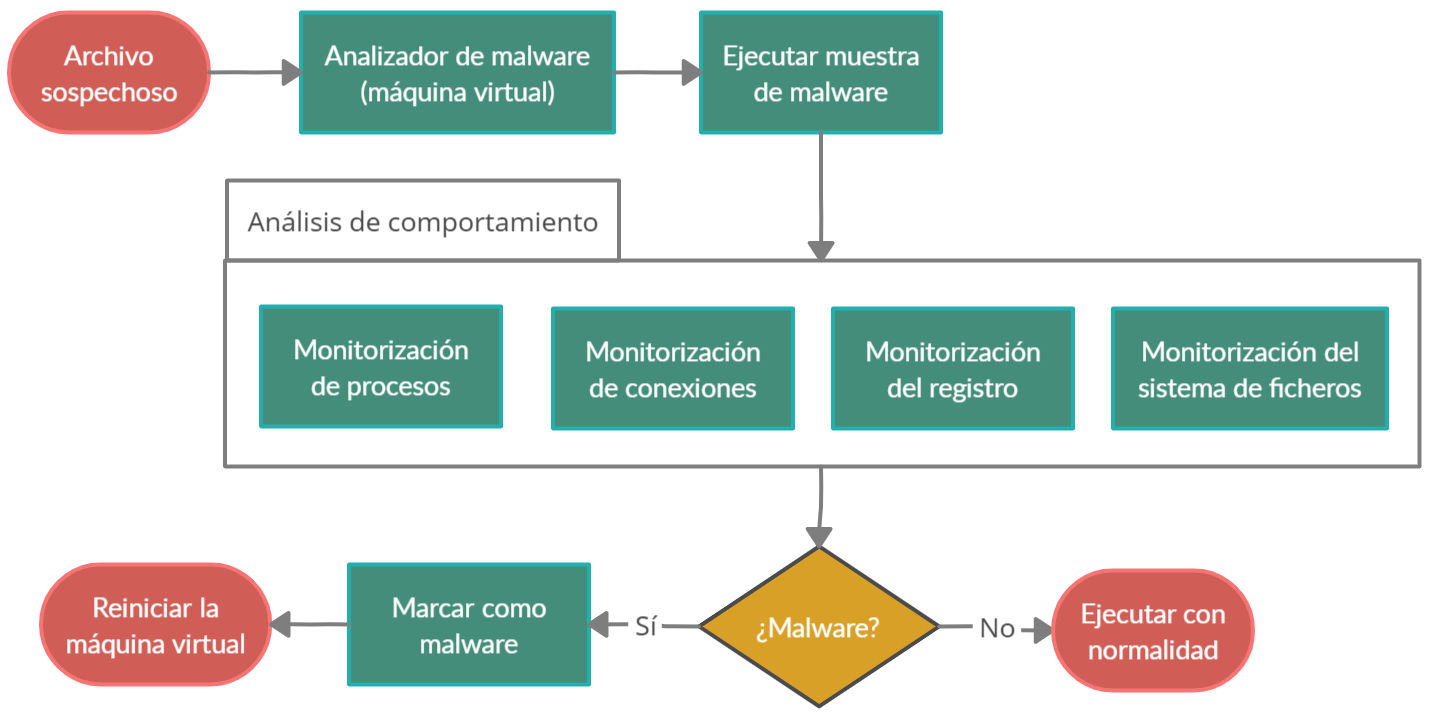
\includegraphics{images/dynamic-flow.png}}}
\end{center}
\caption{Diagrama de flujo de un análisis dinámico.}
\label{fig:dinamFlow}
\end{figure}

\subsection{Herramientas}

\noindent Cuando se habla de las herramientas de análisis dinámico, se puede diferenciar entre análisis dinámico automatizado y análisis dinámico manual. Por lo general, los programas o plataformas web basadas en \textit{sandboxing} pertenecen al análisis automatizado e incluyen monitorización, en cambio, las herramientas de análisis manual implican controlar la información que se quiere obtener de ella y analizarla después. En la Tabla \ref{tab:toolsDin} se muestran las herramientas más utilizadas en el análisis dinámico de malware que no hayan sido explicadas anteriormente.

\begin{table}[htb!]
\centering
\scriptsize %para hacer la tabla mas pequeña
\caption{Herramientas de análisis dinámico.}
\begin{tabular}{|l|p{11.5cm}|}
\hline
\rowcolor[HTML]{C0C0C0}
\multicolumn{1}{|c|}{\cellcolor[HTML]{C0C0C0}{\textbf{Herramienta}}} & \multicolumn{1}{c|}{\cellcolor[HTML]{C0C0C0}{\textbf{Descripción}}}\\ \hline
\textbf{Cuckoo Sandbox}&Herramienta de análisis automatizado de malware de código abierto en Windows, macOS, Linux y Android que utiliza la tecnología de sandboxing. Cuckoo Sandbox tiene un diseño modular, lo que permite personalizar cualquier aspecto del procesamiento del análisis de los resultados, de la generación de informes y del entorno de análisis.\\ \hline
\textbf{Regshot}& Programa que realiza dos instantáneas (una antes de ejecutar el malware y otra después) y las compara encontrando los valores modificados durante la actuación del código malicioso \cite{PMA2012}.\\ \hline
    \textbf{Wireshark}&Herramienta más usada en todo el mundo para analizar el tráfico de red con gran detalle. Soporta gran variedad de plataformas y protocolos y dispone de múltiples filtros, formatos y formas de exportar la información obtenida \cite{WRSKDOC} \cite{92}.\\ \hline
    \textbf{ApateDNS}&Herramienta gratuita que se puede utilizar para encontrar peticiones \gls{DNS} realizadas por un malware. Esto lo hace suplantando respuestas \gls{DNS} a una dirección IP específica escuchando en el puerto 53 \gls{UDP} en la máquina local \cite{PMA2012}.\\ \hline
    \textbf{APIMiner}& Herramienta que registra las llamadas a \gls{API} realizadas durante la actuación de una muestra. El resultado que ofrece es un registro de las llamadas a \gls{API} junto a sus argumentos ordenadas según el momento en el que fueron invocadas \cite{Mohanta2020}.\\ \hline
\end{tabular}
\label{tab:toolsDin}
\end{table}

\begin{comment}
\begin{itemize}
    \item \textbf{Cuckoo Sandbox}: Herramienta de análisis automatizado de malware de código abierto en Windows, macOS, Linux y Android que utiliza la tecnología de \textit{sandboxing}. Cuckoo Sandbox tiene un diseño modular, lo que permite personalizar cualquier aspecto del procesamiento del análisis de los resultados, de la generación de informes y del entorno de análisis.
    \item \textbf{Regshot}: Programa que realiza dos instantáneas (una antes de ejecutar el malware y otra después) y las compara encontrando los valores modificados durante la actuación del código malicioso \cite{PMA2012}.
    \item \textbf{Wireshark}: Herramienta más usada en todo el mundo para analizar el tráfico de red con gran detalle. Soporta gran variedad de plataformas y protocolos y dispone de múltiples filtros, formatos y formas de exportar la información obtenida \cite{WRSKDOC}.
    \item \textbf{ApateDNS}: Herramienta gratuita que se puede utilizar para encontrar peticiones \gls{DNS} realizadas por un malware. Esto lo hace suplantando respuestas \gls{DNS} a una dirección \gls{IP} específica escuchando en el puerto 53 \gls{UDP} en la máquina local \cite{PMA2012}.
    \item \textbf{APIMiner}: Herramienta que registra las llamadas a \gls{API} realizadas durante la actuación de una muestra. El resultado que ofrece es un registro de las llamadas a \gls{API} junto a sus argumentos ordenadas según el momento en el que fueron invocadas \cite{Mohanta2020}.
\end{itemize}
\end{comment}
\subsection{Limitaciones}

\noindent El análisis dinámico es más efectivo que el análisis estático descrito anteriormente y no requiere desensamblar el ejecutable. El punto negativo del análisis dinámico es que el consumo de recursos es mayor y lleva más tiempo, aumentando los problemas de escalabilidad. Por otro lado, a veces el malware está destinado a un cierto sistema o condiciones del mismo (tener un motor de búsqueda concreto, determinadas \gls{DLL}s, etc.), o quizá tenga protección contra máquinas virtuales, lo que podría provocar que no se pueda detectar su comportamiento malicioso en el laboratorio de análisis seguro que se haya montado \cite{Gandotra2014}. En definitiva, lo más efectivo viene a ser combinar tanto el análisis estático como el análisis dinámico para conseguir el mejor resultado posible. La Tabla \ref{tab:tabla2} se muestra de manera clara las diferencias fundamentales entre el análisis el estático y el dinámico, indicando los métodos de análisis que usan cada uno \cite{121}. 

\begin{table}[h!]
\centering
\scriptsize %para hacer la tabla mas pequeña
\caption{Diferencias entre análisis dinámico y estático.}
\begin{tabular}{|l|c|c|}
\hline
\rowcolor[HTML]{C0C0C0}
\multicolumn{1}{|c|}{\cellcolor[HTML]{C0C0C0}{\textbf{Métodos de análisis}}} & \multicolumn{1}{c|}{\cellcolor[HTML]{C0C0C0}{\textbf{Estático}}} & \multicolumn{1}{c|}{\cellcolor[HTML]{C0C0C0}{\textbf{Dinámico}}} \\ \hline
{\color[HTML]{000000} Extracción de cadenas} & {\color[HTML]{000000} Sí} & {\color[HTML]{000000} No} \\ \hline
{\color[HTML]{000000} Secuencias de bytes} & {\color[HTML]{000000} Sí} & {\color[HTML]{000000} No} \\ \hline
{\color[HTML]{000000} Códigos de operación} & {\color[HTML]{000000} Sí} & {\color[HTML]{000000} No} \\ \hline
{\color[HTML]{000000} Llamadas a las \gls{API}} & {\color[HTML]{000000} Sí} & {\color[HTML]{000000} Sí} \\ \hline
{\color[HTML]{000000} Sistema de ficheros} & {\color[HTML]{000000} No} & {\color[HTML]{000000} Sí} \\ \hline
{\color[HTML]{000000} Registros de \gls{CPU}} & {\color[HTML]{000000} Sí} & {\color[HTML]{000000} Sí} \\ \hline
{\color[HTML]{000000} Características del \gls{PE}} & {\color[HTML]{000000} Sí} & {\color[HTML]{000000} No} \\ \hline
{\color[HTML]{000000} Monitorización de la red} & {\color[HTML]{000000} No} & {\color[HTML]{000000} Sí} \\ \hline
{\color[HTML]{000000} Acceso a memoria} & {\color[HTML]{000000} No} & {\color[HTML]{000000} Sí} \\ \hline
{\color[HTML]{000000} Sandboxing} & {\color[HTML]{000000} No} & {\color[HTML]{000000} Sí} \\ \hline
{\color[HTML]{000000} Excepciones} & {\color[HTML]{000000} No} & {\color[HTML]{000000} Sí} \\ \hline
\end{tabular}
\label{tab:tabla2}
\end{table}


\section{Análisis Híbrido}
\label{sec:ahibrido}

\noindent El análisis híbrido es una combinación de las técnicas de análisis estáticas y dinámicas, proporcionando al sistema una mayor seguridad usando ambos enfoques \cite{111}. Este análisis puede detectar malware que está tratando de ocultarse y extraer los indicadores técnicos mediante el análisis estático. Aplica el análisis estático a datos generados por el análisis dinámico en tiempo de ejecución, por lo que, si el malware es cambiante, en análisis dinámico detectaría esto y enviaría los nuevos datos al análisis estático, repitiéndose el ciclo. De esta manera, se generarán indicadores \gls{IoC} de manera más rápida y eficiente \cite{89}. Este enfoque a primera vista parece ser el mejor, ya que combina el análisis estático con el dinámico, pero este no es siempre el caso. Un estudio \cite{120} revela que es poco probable que un enfoque híbrido sea superior al análisis completamente dinámico o estático. Bien es cierto que el análisis híbrido ofrece beneficios en algunos casos, pero en ese trabajo se demuestra que tales afirmaciones deberían estar sujetas a un escrutinio cuidadoso. Además, se debe determinar si estos beneficios existen para el análisis de una amplia gama de muestras de malware o si solo son relevantes para un conjunto reducido de muestras.



\section{Aprendizaje Automático Aplicado al Análisis de Malware}
\label{sec:mlaplicado}


\noindent El aprendizaje automático, en inglés \gls{ML}, es una rama de la inteligencia artificial que permite crear sistemas con la capacidad de identificar patrones de comportamiento y de hacer predicciones de forma autónoma \cite{124}. Esto es posible gracias a algoritmos que analizan una gran cantidad de datos y reconocen patrones para realizar predicciones con nuevos datos sin estar programados para producir un resultado en particular. 
El objetivo final es que el modelo construido aprenda solo de forma que reduzca la implicación del usuario y este realice su tarea de forma independiente \cite{SML2018}. El proceso de construir un modelo sigue ciertos pasos \cite{Thomas_2020}:

\begin{itemize}
    \item \textbf{Recolección de datos}: En esta fase se recogen todos los datos que vayan a ser usados para formar el \textit{dataset} del modelo y se dividen en datos de entrenamiento y datos de prueba. Los primeros serán los utilizados para construir el modelo y los últimos para evaluar el mismo.
    \item \textbf{Preparación de los datos}: Es importante procesar los datos antes de introducirlos al modelo, y para ello, será necesario aplicar una serie de operaciones de transformación y limpieza sobre ellos. Se emplean operaciones como la normalización, la estandarización o la aplicación de expresiones no lineales.
    \item \textbf{Selección del modelo}: Dependiendo del tipo de datos se vayan a utilizar y la finalidad del modelo, se elegirá un modelo de \gls{ML} u otro, ya que existen diversos tipos y cada uno es más adecuado a un tipo de datos o forma de trabajo. Por ejemplo, los modelos de regresión están más destinados a tratar variables continuas.
    \item \textbf{Extracción de características}: El \textit{dataset} utilizado puede tener ciertas variables o características que no sean importantes o determinantes para el modelo, en ese caso, se seleccionaran las necesarias para implementar el modelo de forma que no haya variables redundantes que perjudiquen la precisión del modelo.
    \item \textbf{Entrenamiento del modelo}: Antes de probar e implementar el modelo, será necesario entrenarlo con los datos previamente seleccionados para esta tarea.
    \item \textbf{Prueba del modelo}: En esta fase, se prueba el modelo entrenado con los datos seleccionados para ello.
    \item \textbf{Implementación del modelo}: Por último, se implementa el modelo para su funcionamiento final en tiempo real.
\end{itemize}

En definitiva, el \gls{ML} se utiliza para que los ordenadores, entrenados, tomen sus propias decisiones basándose en un algoritmo, imitando el comportamiento humano. Los algoritmos de \gls{ML} se clasifican en cuatro categorías, que son las siguientes \cite{Thomas_2020}:


\begin{itemize}

    \item \textbf{Aprendizaje supervisado}: Cuando se habla de aprendizaje supervisado, la persona que construye el modelo conoce tanto las variables de entrada como las de salida \cite{MML2018}. La variable de salida es también conocida como la señal de supervisión. Algunos algoritmos usados para este tipo de aprendizaje son los árboles de decisión, el algoritmo \gls{NB} o las máquinas de soporte vectorial (\gls{SVM}) \cite{Thomas_2020}. En la Figura \ref{fig:supervisado} se puede ver un gráfico que muestra el comportamiento descrito.
    
    \begin{figure}[htb]
    \begin{center}
    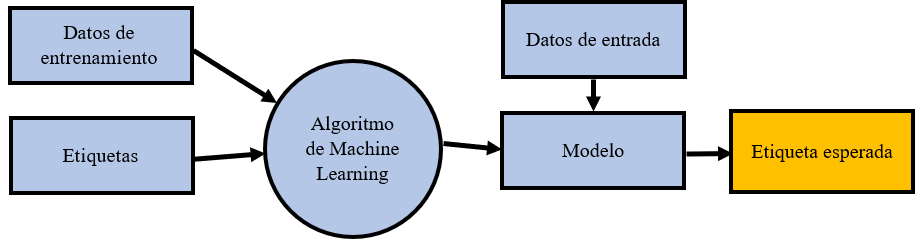
\includegraphics[width=0.80\linewidth]{images/supervisado.PNG}
    \end{center}
    \caption{Modelo de aprendizaje supervisado}
    \label{fig:supervisado}
    \end{figure}
    
    \item \textbf{Aprendizaje no supervisado}: En este tipo de aprendizaje, no se tiene claro cuál será la salida de los modelos \cite{MML2018} y únicamente se conocen los datos de entrada. De esta forma, estos algoritmos intentan encontrar en los datos patrones y clases que puedan ser útiles. Algoritmos comúnmente usados en aprendizaje no supervisado son las redes neuronales o diferentes tipos de agrupamientos (\textit{clustering}) como el algoritmo k-means, normalmente indicado para datos numéricos \cite{Thomas_2020}. En la Figura \ref{fig:nosupervisado} se puede ver un gráfico que muestra el comportamiento descrito.
    
    \begin{figure}[htb]
    \begin{center}
    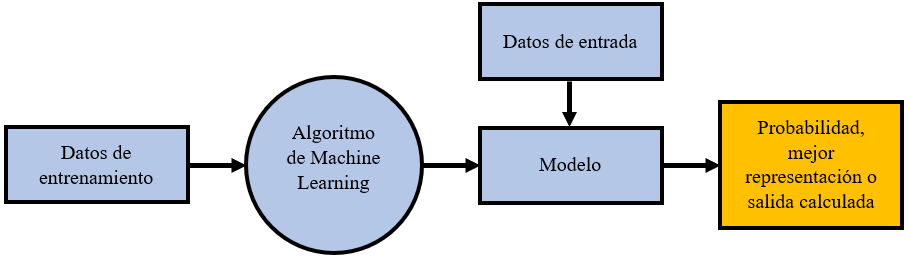
\includegraphics[width=0.80\linewidth]{images/nosupervisado.PNG}
    \end{center}
    \caption{Modelo de aprendizaje no supervisado}
    \label{fig:nosupervisado}
    \end{figure}
    
    \item \textbf{Aprendizaje por refuerzo}: El modelo aprende a base de prueba y error. El modelo (o agente) interactúa con el entorno (contiene las reglas y limitaciones) y va mejorando. El agente, según el estado del entorno, realiza una acción y el entorno responde, entonces, el agente utiliza la información recibida como "recompensa" o "castigo" para orientar su comportamiento de forma que si la respuesta del entorno es positiva (recompensa), el agente reforzará ese comportamiento y si, por el contrario, esta respuesta es negativa (castigo), el agente actuará de forma distinta llegado de nuevo el mismo estado u otro similar \cite{MML2018} \cite{Thomas_2020}. En la Figura \ref{fig:areforzado} se puede ver un gráfico que muestra el comportamiento descrito.
    
    \begin{figure}[htb]
    \begin{center}
    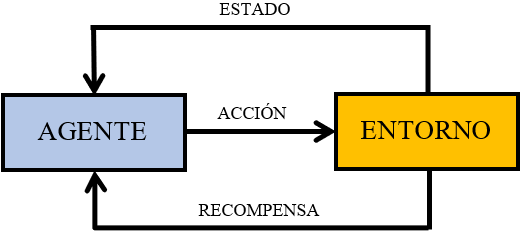
\includegraphics[width=0.45\linewidth]{images/areforzado.PNG}
    \end{center}
    \caption{Modelo de aprendizaje por refuerzo}
    \label{fig:areforzado}
    \end{figure}

     \item \textbf{Aprendizaje semi-supervisado}: El aprendizaje semi-supervisado se aplica cuando una parte de los datos están etiquetados (se conoce la entrada y la salida) y la otra no. Esto puede ocurrir cuando generar datos es un proceso muy costoso \cite{MML2018}. En estos casos, el problema se encuentra entre el aprendizaje supervisado y el no supervisado y se aplican algoritmos como modelos generativos (\textit{generative models}) o métodos basados en gráficos (\textit{graph-based methods}) o máquinas de soporte vectorial semi-supervisadas \cite{Thomas_2020}.
    
\end{itemize}

La utilización de estos tipos depende de las necesidades y del problema que se quiera resolver; en el caso del análisis de malware, el aprendizaje supervisado es el más usado \cite{zero}.

\subsection{Aprendizaje Supervisado}\label{sec:algoritmos}
\noindent La característica que define al aprendizaje supervisado es la disponibilidad de datos de entrenamiento etiquetados. El nombre indica una idea de un ``supervisor'' que instruye al sistema con etiquetas para que pueda asociarlas con los datos de entrada y que posteriormente sea capaz de clasificar otros datos no etiquetados \cite{126}.

El aprendizaje supervisado se puede dividir en dos tipos: clasificación y regresión. Los modelos de regresión se basan en el análisis de relaciones entre tendencias y variables para poder realizar predicciones sobre variables continuas, y los de clasificación asignan etiquetas discretas a observaciones particulares \cite{127}. A continuación, se describirán de forma general los algoritmos de clasificación de aprendizaje supervisado más utilizados en análisis de malware:


\begin{itemize}
\item \textbf{Regresión logística (\gls{LR})}: Es comúnmente empleado para los sistemas de puntuación en aplicaciones y para el modelado de riesgo crediticio \cite{131}. En primer lugar, se realiza una regresión lineal sobre la relación entre variables para obtener el modelo. Después, la función logística se aplicará a la regresión para obtener la probabilidad de que la muestra pertenezca a cada una de las clases y se clasificará en función de la probabilidad más alta. La función logística, también llamada función \textit{sigmoidea}, es una curva en forma de ``S'' que toma cualquier número lo asigna a un valor entre 0 y 1, pero nunca esos valores exactamente \cite{132}. Los trabajos que usan este algoritmo para sus análisis son: \cite{elderan}, \cite{rwguard} y \cite{entropy}.

Para realizar las predicciones, hay que tener en cuenta que la probabilidad debe de transformarse en valores binarios (0 o 1), y para ello se introduce en la ecuación de regresión logística junto con los coeficientes (valores beta) del algoritmo, estimados mediante el método de máxima verosimilitud \cite{133}. Los mejores coeficientes darán como resultado un modelo que prediga un valor muy cercano a 1 para una clase y 0 para la otra.

Para obtener la función de regresión logística se usa la Fórmula \ref{equ:lr} \cite{132}
\begin{equation}\label{equ:lr}
y = \frac{e^{(\beta_0 + \beta_1x)}}{1 + e^{(\beta_0 + \beta_1x)}}
\end{equation}
\noindent donde, $y$ el valor de salida previsto, $\beta_0$ el coeficiente de sesgo o intersección y $\beta_1$ el coeficiente para cada valor de entrada $x$


La Figura \ref{fig:logistic} representa gráficamente todo lo explicado anteriormente. 

\begin{figure}[h!]
\begin{center}
{\scalebox{.7}{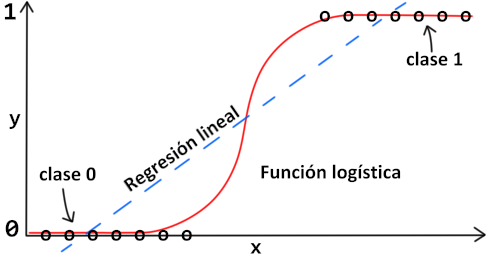
\includegraphics{images/logistic.png}}}
\end{center}
\caption{Gráfico de la regresión logística.}
\label{fig:logistic}
\end{figure}


\item \textbf{Bayesiano ingenuo (\gls{NB})}: Es un clasificador basado en el teorema de Bayes. Almacena la probabilidad previa de cada clase y la probabilidad condicional de cada valor de los atributos. Estima estas cantidades contando la frecuencia de ocurrencia de las clases y de los atributos en los datos de entrenamiento. Después, asumiendo la independencia condicional de los atributos, usa la regla de Bayes para calcular la probabilidad posterior de cada clase dados nuevos datos sin etiquetar \cite{134}. Los trabajos que usan este algoritmo son: \cite{elderan}, \cite{flow}, \cite{shallow}, \cite{rwguard}, \cite{detecting} y \cite{Kok2019}.

Para calcular la probabilidad posterior de la clase se usa la Fórmula \ref{equ:nb} \cite{131}
\begin{equation}\label{equ:nb}
P (clase | datos) = \frac{P (datos | clase)*P (clase)}{P (datos)}
\end{equation}
\noindent donde, $P(clase)$ es la probabilidad previa de una etiqueta, $P(datos | clase)$ es la probabilidad previa de que un conjunto de características dado se clasifique como etiqueta y $P(datos)$ es la probabilidad previa de que apareciera un conjunto de características.


\item \textbf{K-vecinos más cercanos (\gls{KNN})}: Este algoritmo de aprendizaje perezoso clasifica los datos en función de su proximidad con otros mediante funciones de distancia \cite{136}. Ser un algoritmo perezoso significa que no se necesita generalizar los datos de entrenamiento para la generación del modelo \cite{137}. En \gls{KNN}, la ``K'' es el número de vecinos más cercanos y es conveniente que sea impar si hay un número par de clases. Para seleccionar la ``K'' adecuada, se ejecuta el algoritmo \gls{KNN} varias veces con diferentes valores de ``K'' y se elige el valor que reduzca la cantidad de errores y mantenga la capacidad del algoritmo para hacer predicciones con precisión con datos nuevos. La principal desventaja ese algoritmo es que se vuelve más lento a medida que aumenta el número de datos \cite{135}. Los trabajos que usan este algoritmo para construir sus modelos de \gls{ML} son: \cite{shallow} y \cite{detecting}.

La distancia entre los k vecinos se puede calcular con la Fórmula de distancia euclidiana \ref{equ:knn} \cite{143}
\begin{equation}\label{equ:knn}
d(p,q) = \sqrt{\sum_{i=1}^{n} (q_i - p_i)^2}
\end{equation}
\noindent donde, $p$ y $q$ son la posición de dos vecinos cualquiera, $d$ la distancia que queremos calcular y $n$ el número de dimensiones o características.

En la Figura \ref{fig:knn} se puede ver una representación gráfica del algoritmo.

\begin{figure}[h!]
\begin{center}
{\scalebox{.65}{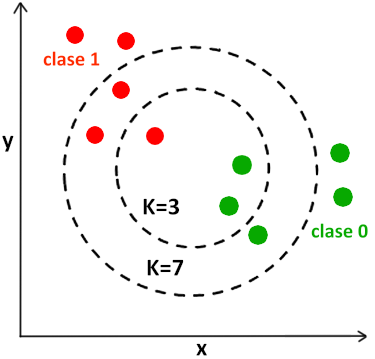
\includegraphics{images/knn.png}}}
\end{center}
\caption{Representación gráfica del algoritmo KNN.}
\label{fig:knn}
\end{figure}

\item \textbf{Árboles de decisión (\gls{DT})}: Proporciona una partición jerárquica de los datos de entrenamiento, donde las 'hojas' o nodos del árbol representan etiquetas y las ramas representan las características o atributos de los datos \cite{141}. El conjunto de datos es dividido en subconjuntos cada vez más pequeños, y esto se repite de manera recursiva hasta que ya no haya más datos por analizar o se cumplan ciertas condiciones, como una profundidad límite. Sigue la estructura del algoritmo \gls{ID3} para determinar la división de los datos \cite{142}. Los trabajos que usan este algoritmo para sus análisis son: \cite{shallow}, \cite{rwguard} y \cite{detecting}.

El algoritmo \gls{ID3} selecciona la mejor característica mientras construye el árbol de decisión. Para esta elección, se usa una métrica llamada mérito o \textit{information gain}, que calcula la reducción de la entropía \cite{144}. La característica con el mayor mérito será la mejor. El mérito de una característica se calcula con la Fórmula \ref{equ:merito}
\begin{equation}\label{equ:merito}
IG(S,a) = E(S) - E(S | a)
\end{equation}
\noindent donde, $IG(S,a)$ es el mérito para el conjunto de datos $S$ para la característica de la columna $a$, $E(S)$ es la entropía del conjunto de datos antes de cualquier cambio y $E(S | a)$ es la entropía condicionada por $a$.


%\st{Para obtener la entrop\'ia se usa la siguiente f\'ormula, donde...} %\textit{E} es la entropía que queremos calcular del es el conjunto de datos o \textit{dataset} \textit{S}, \textit{n} el número total de clases en la columna de destino y \(p_i\) la probabilidad de la clase \textit{i} o la relación entre el número de filas con clase \textit{i} en la columna de destino y el número total de filas en el conjunto de datos \cite{142}:
%\change{modificar el estilo de describir las f\'ormulas por el siguiente. 
%Unificar t\'erminos F\'ormula o Ecuaci\'on utilizas \$ en vez de el comando textit - HECHO}

Para obtener la entropía se usa la Fórmula \ref{equ:entropy} \cite{142}
%\[ E(S) = \sum_{i=1}^{n} - p_i\log_2(p_i) \]
\begin{equation}\label{equ:entropy}
E(S) = \sum_{i=1}^{n} - p_i\log_2(p_i)
\end{equation}
\noindent donde, $E$ es la entropía que queremos calcular del es el conjunto de datos $S$, $n$ el número total de clases en la columna de destino y $p_i$ la probabilidad de la clase $i$ o la relación entre el número de filas con clase $i$ en la columna de destino y el número total de filas del conjunto de datos.

En la Figura \ref{fig:tree} se puede ver un ejemplo de un árbol de decisión sobre préstamos.

\begin{figure}[h!]
\begin{center}
{\scalebox{.34}{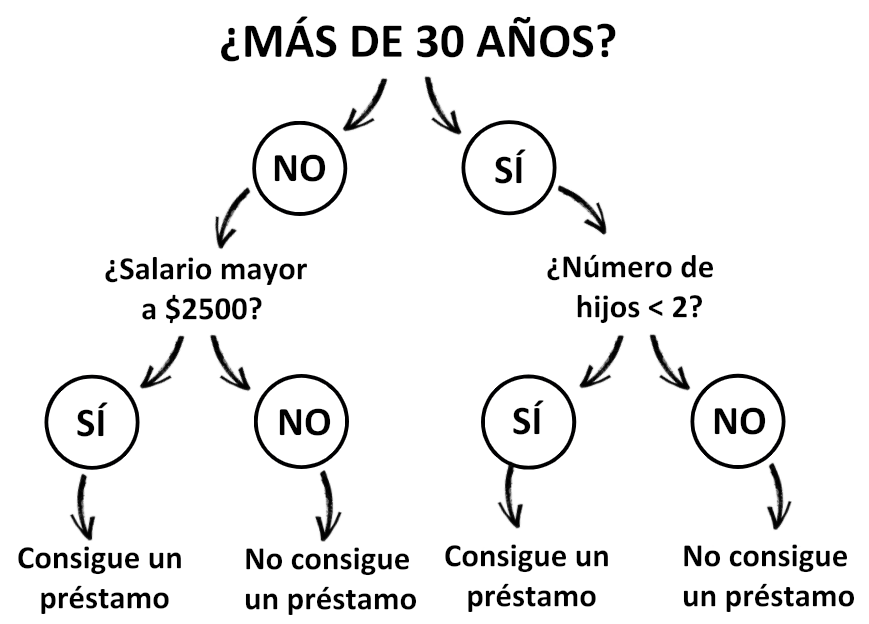
\includegraphics{images/tree.png}}}
\end{center}
\caption{Representación gráfica de un árbol de decisión.}
\label{fig:tree}
\end{figure}

\newpage

\item \textbf{Bosque aleatorio (\gls{RF})}: Como sugiere el nombre, un bosque aleatorio es la fusión de valores aleatorios provenientes de un conjunto de árboles de decisión \cite{138}. Estos árboles de decisión están generalmente entrenados con el método de \textit{``bagging''}, que consiste en la combinación de modelos de aprendizaje para aumentar la precisión del resultado final \cite{140}. Una ventaja de este algoritmo es que se puede utilizar para problemas de clasificación y también para problemas de regresión. Los trabajos que hacen uso de este algoritmo son: \cite{flow}, \cite{traffic}, \cite{sdn}, \cite{rwguard}, \cite{detecting} y \cite{Kok2020}.
%\change{ordenar por fecha las citas ..17, ..18, ..18a, ..19 - HECHO}
Para elegir los valores aleatorios, se buscará la mejor característica en un conjunto aleatorio de características. Se pude incrementar la aleatoriedad aún más mediante el uso de umbrales para cada característica en lugar de buscar las mejores \cite{139}.

La Figura \ref{fig:RF} es una representación gráfica del algoritmo con dos árboles de decisión.

\begin{figure}[h!]
\begin{center}
{\scalebox{.29}{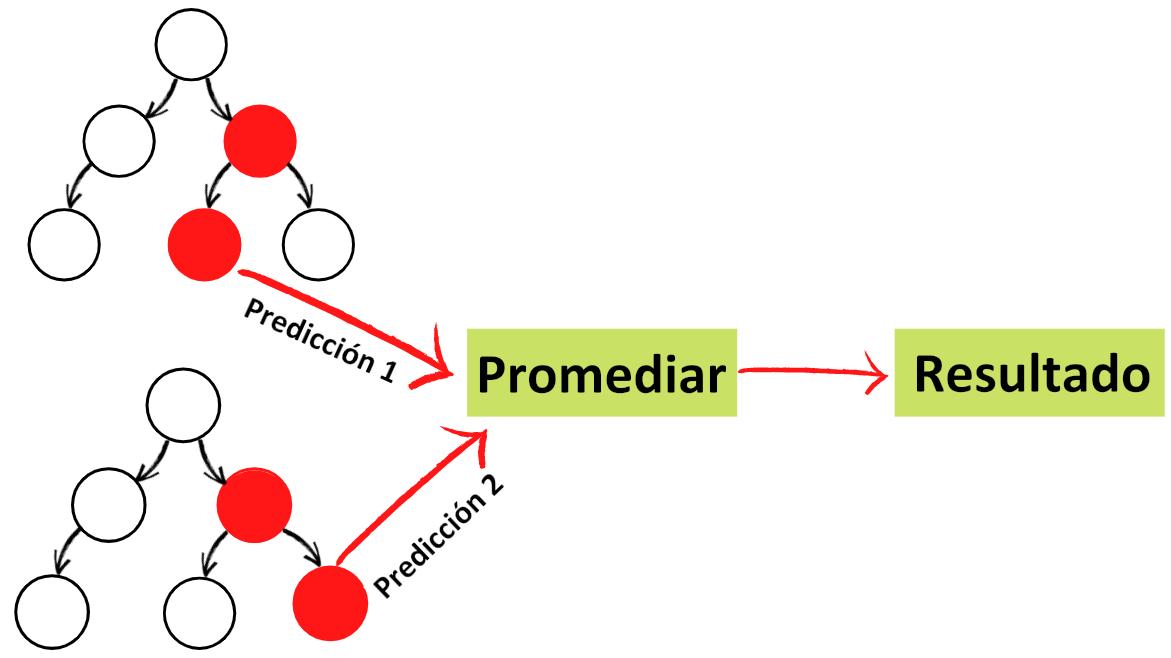
\includegraphics{images/rf.png}}}
\end{center}
\caption{Representación gráfica del algoritmo Bosque Aleatorio.}
\label{fig:RF}
\end{figure}


Para promediar los resultados, se utiliza la Fórmula \ref{equ:rf} \cite{145}
\begin{equation}\label{equ:rf}
RFfi_i = \frac{\sum_{j \in n} normfi_{ij}}{T}
\end{equation}
\noindent donde, $T$ es el número de árboles de decisión, $RFfi_i$ la importancia de la característica $i$ calculada a partir de todos los árboles de decisión $n$ y $normfi_{ij}$ la importancia de la característica $i$ normalizada en el árbol de decisión $j$.


\item \textbf{Máquina de soporte vectorial (\gls{SVM})}:
Una máquina de soporte vectorial clasifica los datos mediante la construcción de un plano de decisión (hiperplano) de N dimensiones que separa los datos en dos categorías, dependiendo de sus características \cite{131}. Los modelos \gls{SVM} están relacionados con las redes neuronales, ya que un modelo que utilice una función sigmoide es equivalente a una red neuronal de perceptrón de dos capas \cite{128}. Un conjunto de características junto con sus etiquetas, que representan las categorías, se llama vector. El objetivo del \gls{SVM} es encontrar el hiperplano óptimo que separe a los vectores según sus categorías. Los trabajos que usan este algoritmo para sus análisis son: \cite{elderan}, \cite{flow}, \cite{shallow}, \cite{detecting} y \cite{entropy}.

Los vectores cercanos al hiperplano se llaman vectores de apoyo, y la distancia entre estos vectores de apoyo se llama margen o \textit{maximal margin} \cite{146}. Es difícil separar datos perfectamente en dos categorías, por lo que se puede permitir cierta flexibilidad en la clasificación con los denominados márgenes blandos o \textit{soft-margins}, introduciendo un nuevo parámetro \textit{c} en la máquina.

\gls{SVM} utiliza un conjunto de funciones matemáticas que se definen como el núcleo o kernel, el cual procesa los datos de entrada y devuelve el producto interno entre dos puntos en un espacio de características de cualquier dimensión \cite{147}. Si los datos se pueden separar con un hiperplano lineal, usamos \gls{SVM} Lineal con kernel lineal. Si ese no es el caso, debemos recurrir a \gls{SVM} No Lineal y usar kernels para transformar espacios no lineales en espacios lineales \cite{148}.

Los diferentes algoritmos de \gls{SVM} utilizan diferentes tipos de kernel. Los más comúnmente usados son los siguientes con sus respectivas ecuaciones: 

\begin{itemize}
    \item \textbf{Lineal}: El más simple de todos, calculado con la Fórmula \ref{equ:l} \cite{150}
    \begin{equation}\label{equ:l}
    k(x_i,x_j) = (x_ix_j+c)
    \end{equation}
    \noindent donde, $(x_i,x_j)$ son los dos puntos en el espacio de características y $c$ es el parámetro de flexibilidad.
    
    \item \textbf{Polinómico}: Usado en el procesamiento de imágenes y calculado con la Fórmula \ref{equ:p} \cite{149}
    \begin{equation}\label{equ:p}
    k(x_i,x_j) = (\alpha x_ix_j+c)^d
    \end{equation}
    \noindent donde, $(x_i,x_j)$ son los dos puntos en el espacio de características, $d$ es el grado del polinomio, $\alpha$ la pendiente y $c$ un parámetro que intercambia la influencia de los términos de orden superior frente a los de orden inferior en el polinomio. Si $c = 0$, el kernel se denomina homogéneo.
    
    \item \textbf{Función de base radial Gaussiana}: Utilizado cuando no hay conocimiento previo sobre los datos y calculado con la Fórmula \ref{equ:rg} \cite{147}
    \begin{equation}\label{equ:rg}
    k(x_i,x_j) = \exp(-\gamma \vert\vert x_i-x_j \vert\vert^2)
    \end{equation}
    \noindent donde, $(x_i,x_j)$ son los dos puntos en el espacio de características y $\gamma$ es la función \gls{RBF}.
    
    \item \textbf{Sigmoide}: Usada para las redes neuronales y calculada con la Fórmula \ref{equ:s} \cite{150}
    \begin{equation}\label{equ:s}
    k(x_i,x_j) = \tanh(\alpha x_ix_j + c)
    \end{equation}
    \noindent donde, $(x_i,x_j)$ son los dos puntos en el espacio de características y $\alpha$ es la pendiente.
\end{itemize}


La  Figura \ref{fig:SVM} muestra una representación gráfica de un ejemplo de \gls{SVM} lineal de dos dimensiones:

\begin{figure}[h!]
\begin{center}
{\scalebox{.3}{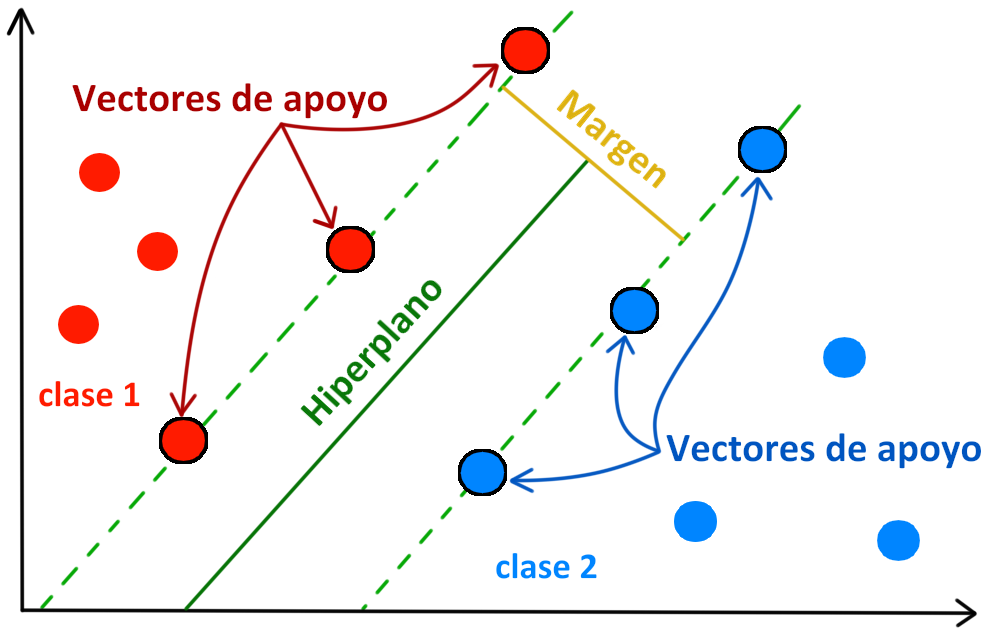
\includegraphics{images/svm.png}}}
\end{center}
\caption{Representación gráfica de SVM lineal de dos dimensiones.}
\label{fig:SVM}
\end{figure}
%\change{unificar el tipo de letra de alas figuras - HECHO}

\end{itemize}

A continuación, se listan las librerías de Python más utilizadas para desarrollar un modelo de \gls{ML}: 

\begin{itemize}
    \item \textbf{Numpy}: Se trata de una de las librerías numéricas más utilizadas para llevar a cabo tanto operaciones matemáticas y lógicas, como ordenado, selección,transformaciones y operaciones estadísticas  sobre \textit{arrays}. Proporciona cantidad de funcionalidades de álgebra lineal, muy útiles en \gls{ML}. Se trata de una librería cuyas operaciones se realizan con gran rapidez, debido a la vectorización: no existe ninguna clase de bucle, indexado, etc. en el código, sino que estas partes más costosas se encuentran por debajo en código C pre-compilado \cite{NMPYDOC}. 
    
    \item \textbf{TensorFlow}: Es una interfaz para expresar algoritmos de \gls{ML}, y una implementación para ejecutarlos. Es un sistema flexible con capacidad para la utilización de una gran cantidad de algoritmos, así como para sistemas heterogéneos y diferentes dispositivos, incluidos móviles, desarrollado por Google \cite{45166}.
    
    \item \textbf{Keras}: Esta librería es muy utilizada para implementar modelos de \textit{deep learning}. Está construida encima de TensorFlow, lo que hace que sea sencilla de utilizar \cite{MML2018}.
     
    \item \textbf{Pandas}: Pandas es un herramienta para explorar, limpiar y procesar datos tabulares, como bases de datos, convirtiéndolos en un tipo de datos concreto, mucho más fácil de manejar, denominado \textit{DataFrame}. Es ampliamente utilizada en modelos de \gls{ML} para obtener una entrada de datos eficiente y eficaz \cite{PNDSDOC}. 
    
    \item \textbf{Matplotlib}: Es una librería utilizada en el campo de la ciencia de datos para visualizar los datos gráficamente. Este aspecto es muy importante para obtener conocimiento de los datos y para razonar los resultados que ofrece el modelo de \gls{ML} \cite{MML2018}.
    
    \item \textbf{Scikit-learn}: Se trata de una librería que proporciona herramientas de \gls{ML} con un entorno para usuarios que no sean expertos. Está enfocada para un uso de propósito general mediante lenguaje de alto nivel. Destaca por su eficiencia, accesibilidad y reusabilidad en varios contextos \cite{sklearn_api}.

\end{itemize}

\subsection{Aplicación del Aprendizaje Automático al Análisis de Malware}

\noindent Cuando se habla del aprendizaje automático en el análisis de malware, es preciso saber que existen diferentes objetivos posibles a conseguir, distintas características a utilizar y cómo extraerlas y el tipo de algoritmo de aprendizaje automático que se utiliza.

Primero, es necesario saber cuál es el objetivo del análisis, que puede ser: la detección de malware (el principal y predominante) para determinar si una muestra es maliciosa; el análisis de similitudes, para estudiar la evolución o variación de las muestras o detectar la pertenencia de una muestra desconocida a una familia; o la detección de categorías de malware, para conocer el objetivo del malware.

Dependiendo del objetivo y del conjunto de datos que se tenga, se hará uso de un tipo concreto de algoritmo de \gls{ML} \cite{Ucci2019}. Esto se puede ver reflejado en el esquema que se muestra en la Figura \ref{fig:esquemaml}.

\begin{figure}[htb!]
\begin{center}
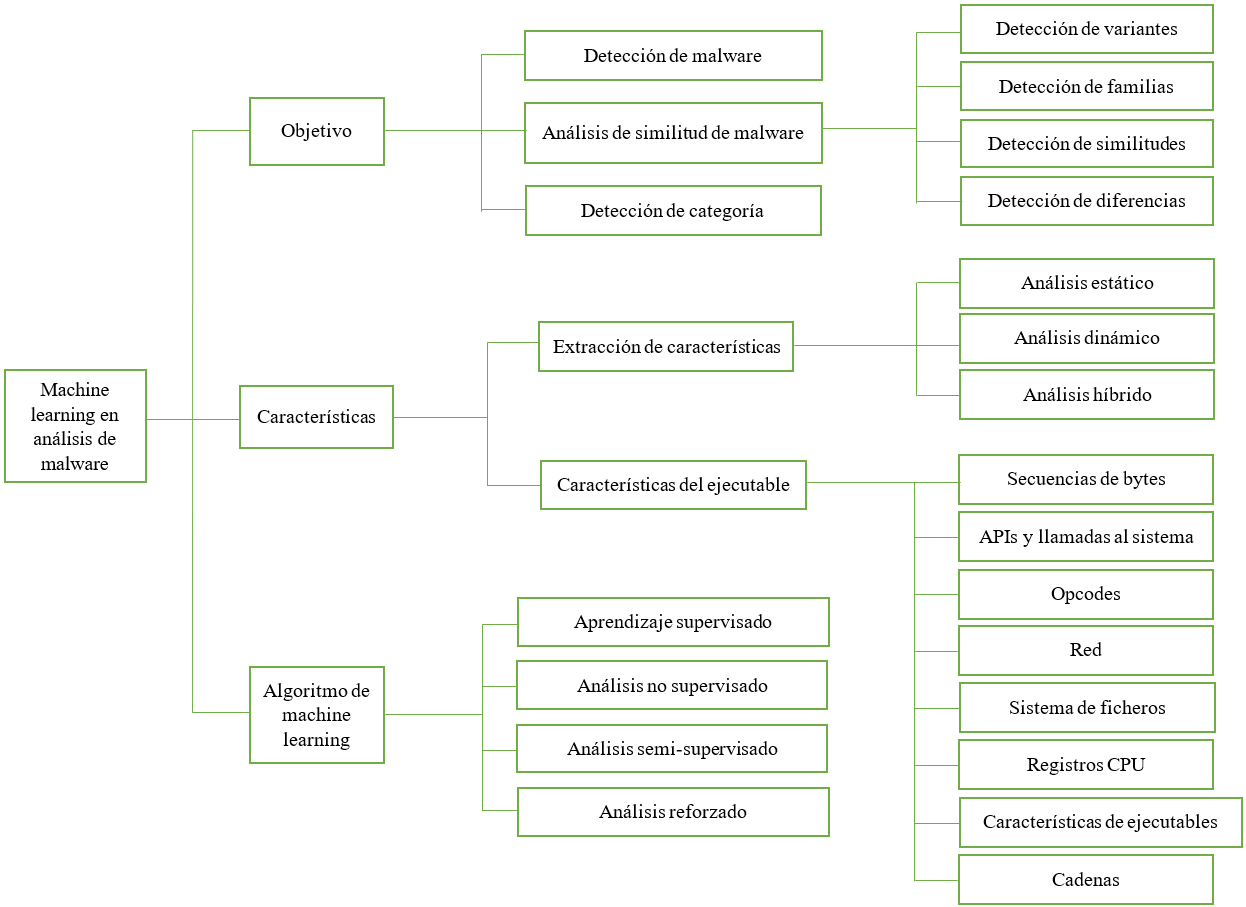
\includegraphics[width=1\linewidth]{images/esquemaml.PNG}
\end{center}
\caption{Taxonomía de las técnicas de ML en el análisis de malware \cite{Ucci2019}}
\label{fig:esquemaml}
\end{figure}

Es importante también conocer las características del ejecutable que se van a utilizar para el análisis, como pueden ser secuencias de bytes, llamadas al sistema y \gls{API}s, actividad de red o cadenas. Todas estas características se extraerán haciendo uso del análisis estático (Sección \ref{sec:aestatico}), del análisis dinámico (Sección \ref{sec:adinamico}) o de la combinación de ambos.

En el caso del análisis de malware y de este trabajo, que está enfocado en detectar programas ransomware, usar un modelo de clasificación es lo más conveniente.
